\documentclass[palatino]{ist-report}

%%%%%%%%%%%%%%%% BEGIN PREAMBLE %%%%%%%%%%%%%%%%
\graphicspath{{graphics/}}

\usepackage{siunitx}

%\usepackage{tikz}
%\usepackage{pgfplots}
%\usetikzlibrary{arrows.meta,positioning}
%\pgfplotsset{compat=1.16, table/search path = {data}}

\usepackage{enumitem}

\usepackage{minted}
\definecolor{bg}{rgb}{0.95,0.95,0.95}
\setminted{linenos, bgcolor = bg, breaklines}
\setmintedinline{bgcolor = {}}
%%%%%%%%%%%%%%%%% END PREAMBLE %%%%%%%%%%%%%%%%%

\settitle{Sistemas Aviónicos Integrados}

\begin{document}

\begin{titlepage}

\begin{center}
	\vspace*{0.05\textheight}
	
\includegraphics[width = 0.4\linewidth, trim = {172.4pt 202.7pt 172.6pt 201.4pt}, clip]{IST_A_CMYK_POS}
	
	\vspace*{0.1\textheight}
	{\huge\bfseries Desenho de um \textit{Primary Flight Display}}
	
	\vspace*{0.03\textheight}
	{\Large Projeto Final de Sistemas Aviónicos Integrados}
	
	\vspace{\fill}
	{\Large \begin{tabular}{l r} Pedro Afonso & \textbf{66277} \\ João Manito & \textbf{73096} \\ Daniel de Schiffart & \textbf{81479}\end{tabular}}
	
	\vspace*{30mm}
	{\large Sistemas Aviónicos Integrados}
	
	\vspace*{0.005\textheight}
	{\Large\itshape Mestrado Integrado em Engenharia Aeroespacial}
	
	\vspace*{0.005\textheight}
	{\large\scshape Instituto Superior Técnico}
	
	\vspace*{0.6cm}
	{\large\bfseries 2018/2019}
\end{center}

\end{titlepage}
\setcounter{page}{1}

\begin{abstract}
    Neste projeto final da unidade curricular de Sistemas Aviónicos Integrados foi desenhado e simulado um \textit{Primary Flight Display} para processar um conjunto de dados de uma simulação de voo em tempo real e simular o comportamento de um verdadeiro \textit{Primary Flight Display} durante o voo simulado.
    
    O \textit{Primary Flight Display} foi desenhado em C com recurso à API OpenGL e à biblioteca gráfica SDL para criar a interface gráfica.
\end{abstract}

{\hypersetup{linkcolor = {black}}\tableofcontents}

\pagebreak

\section{Introdução}

Um \textit{Primary Flight Display}, doravante referido por PFD, é um instrumento de voo moderno desenhado digital que faz recurso a monitores para passar informação ao piloto sobre vários dados do estado atual da aeronave para auxiliar na navegação. Dependendo dos dados mostrados no ecrã e do número de ecrãs presente, o PFD é desenhado para substituir os instrumentos \textit{clássicos} de uma aeronave, com vários mostradores para dados diferentes, por um só mostrador que mostra todos os dados no mesmo sítio.

O nosso projeto foi desenhar um PFD que pudesse mostrar a altitude, velocidade, e atitude de uma aeronave. Para tal, tomámos como exemplo o PFD visível na figura \ref{fig:pfd_example}.
\begin{figure}[ht]
    \centering
    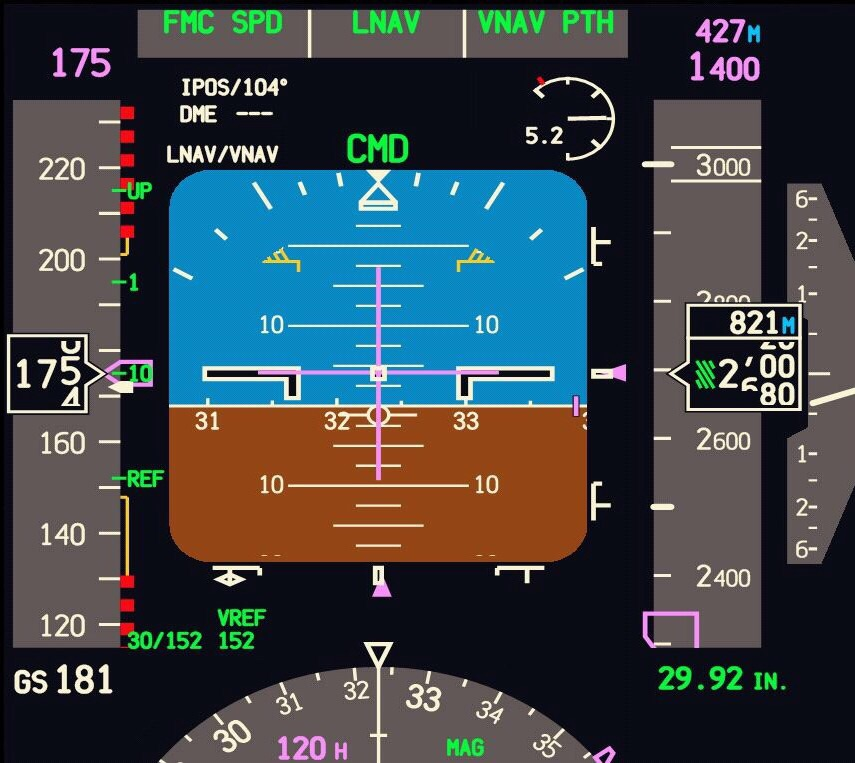
\includegraphics[width = 0.8\linewidth]{pfd_example.png}
    \caption{Exemplo de um PFD comercial, neste caso de um Boeing 747.}
    \label{fig:pfd_example}
\end{figure}

A decisão do uso da linguagem C e de OpenGL veio de um critério que o nosso grupo estableceu no início do projecto: o código ser \textit{low-level} e capaz de ser implementado em diferentes sistemas, com diferentes capacidades.

\subsection{Dados a ser apresentados}\label{sec:data_to_show}

Os dados a serem mostrados foram definidos no enunciado do projeto, e utilizando a figura \ref{fig:pfd_example} como referência também foram implementados mais mostradores no ecrã para além dos requeridos.

Os dados a mostrar foram
\begin{itemize}
    \item A altitude;
    \item A velocidade IAS (\textit{Indicated Airspeed});
    \item A velocidade vertical;
    \item A orientação do avião, incluindo os ângulos de
    \begin{itemize}
        \item \textit{pitch}, ou ângulo de picada;
        \item \textit{roll}, ou ângulo de rolamento;
    \end{itemize}
    \item A orientação magnética do avião.
\end{itemize}

\section{Interface Gráfica}

Utilizamos a linguagem C para programar o display e as bibliotecas gráficas \textit{OpenGL} e SDL. As seguintes funções descritas neste capítulo estão no ficheiro \texttt{draw\_functions.c}, com excepção das funções criadas para desenhar texto e dígitos que se encontram no \texttt{font.c}.

O exemplo do produto final é visível na figura \ref{fig:display_main} e será utilizado como referência visual para esta secção.
\begin{figure}[ht]
    \centering
    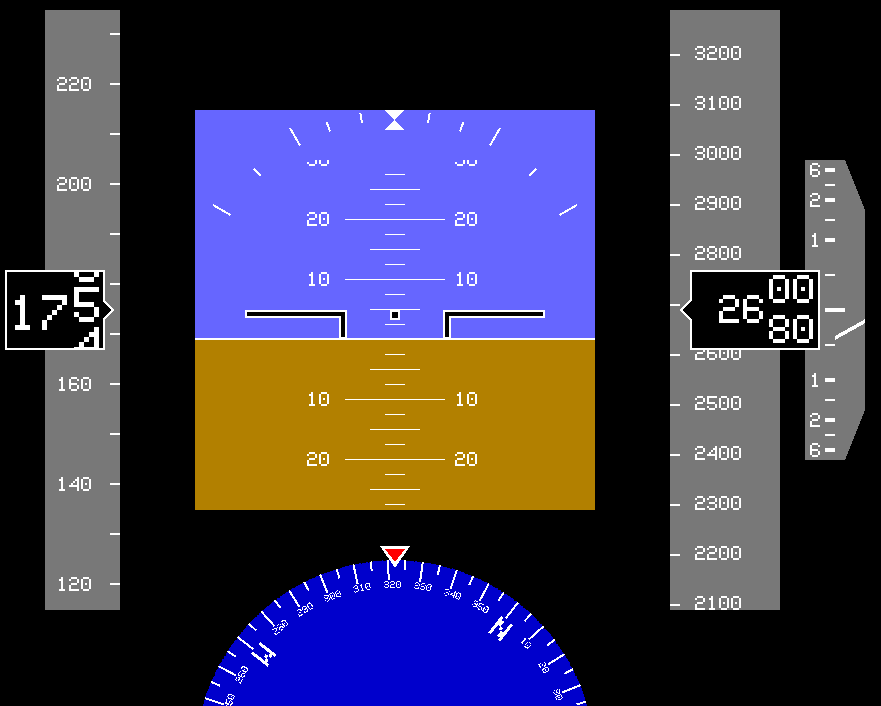
\includegraphics[width = 0.8\linewidth]{PFD_simulado.png}
    \caption{Aspeto final do \textit{display} desenvolvido.}
    \label{fig:display_main}
\end{figure}

\subsection{Horizonte Artificial}
Em primeiro lugar implementamos no PFD o azimute e rolamento em função dos respectivos ângulos. A função chamada:   
\begin{minted}{c}
void draw_artificial_horizon(float pitch, float roll)
\end{minted}
recebe os dois ângulos no tipo \mintinline{c}{float}, para várias casas decimais. Foram criadas as funções com o \texttt{glBegin ( GL\_POLYGON )} para desenhar a parte castanha relativa à terra e a azul relativa ao céu, sendo que os vértices destes dois polígonos variam conforme o ângulo de picada. Para rodar o \textit{display} conforme o ângulo de rolamento desejado, foram usadas as funções \texttt{glTranslatef(midX-50, midY,1.0)} e \texttt{glRotatef (roll , 0 , 0 , 1)}, sendo que a primeira tem o objectivo de nos deslocar para o centro do referencial, ponto de referência para o qual queremos efectuar a rotação com a segunda função mencionada. De notar que \textit{roll} refere-se ao simétrico do ângulo de rolamento, como definido no ficheiro \texttt{comms.c}, devido a este ser definido no sentido anti-horário, e as rotações em openGL serem no sentido horário.

As linhas horizontais referentes aos vários ângulos de picada da aeronave podem tomar posições diferentes, estando estas dependentes do ângulo de picada, mas os indicadores das asas e nariz do avião mantêm-se estáticas. Foi utilizado o comando \texttt{glBegin(GL\_LINES)} em que os vértices de cada linha são definidos em função do pitch. Com vários ciclos conseguimos gerar as linhas necessárias. Para exemplificar:
\begin{minted}{c}
glBegin(GL_LINES);
    glColor3f(1,1,1);
    //10 degree lines
    for (i=1; i<=9; i=i+1){
        //Negative pitch
        glVertex3f(-50,-60*i+pitch_pixels,0);
        glVertex3f(50,-60*i+pitch_pixels,0);

        //Positive pitch
        glVertex3f(-50,60*i+pitch_pixels,0);
        glVertex3f(50,60*i+pitch_pixels,0);
        }

\end{minted}

O PFD programado tem um limite de valores aceites para o ângulo de picada: $90$ graus para o máximo e $-90$ graus para o mínimo. 

\subsection{Indicador de Rolamento}
Para as linhas de indicador de ângulo de rolamento fizemos de maneira oposta, com um arco fixo, mas com um indicador que varia conforme o ângulo de rolamento. Foi usada a função \texttt{glRotatef(i,0,0,1)}, que faz a rotação à volta de um certo ponto, mas com o objectivo de desenhar as linhas do arco com os valores do \textit{roll} através de um ciclo. 

O código que faz o indicador rodar para o \textit{roll} em que a aeronave se encontra, também utiliza a função \texttt{glRotatef(roll,0,0,1)}, mas como é perceptível, a variável agora usada mudou para o ângulo que queremos medir. O indicador é desenhado na forma de triângulo, usando o \texttt{glBegin(GL\_TRIANGLES)} e definindo os seus vértices e a cor. Outro triângulo desenhado na parte superior do arco, serve apenas para indicar o ângulo de rolamento 0. Para demonstração deste caso e também para outros utilizados noutra parte do projecto, é mostrado aqui o exemplo:
\begin{minted}{c}
    glBegin(GL_TRIANGLES);
    glColor3f(1,1,1);
    glVertex3f(-10,0,0);
    glVertex3f(10,0,0);
    glVertex3f(0,10,0);
    glEnd();
\end{minted}

Os limites para o indicador de rolamento, ou seja, os valore que o nosso PFD pode aceitar estão entre $-60$ graus (mínimo) e $60$ graus (máximo).  


\subsection{Indicador de Velocidade}
O Indicador de velocidade mostra a \textit{Indicated Air Speed} em nós.
A função foi definida por:
\begin{minted}{c}
void draw_airspeed_indicator(float airspeed)
\end{minted}
Consiste numa barra lateral do lado esquerdo, estática como \textit{background}, mas com valores amovíveis verticalmente, de acordo com o valor recebido pela função, \textit{IAS} do tipo \mintinline{c}{float} para valores decimais. Ou seja, esta barra funciona como uma espécie de janela para outra superfície, onde estão desenhados os valores de \textit{IAS} e que esta sim, movimenta-se de forma a que o valor que se encontra momentaneamente na centro vertical da janela, represente a \textit{IAS} da aeronave nesse instante. Portanto criamos uma função para movimento de todos os pixeis contidos dentro da janela. O uso deste tipo de janelas é frequente no nosso PFD, para este caso específico temos:

\begin{minted}{c}
    glEnable(GL_SCISSOR_TEST);
    glScissor(50,100,100,600);    
\end{minted}

Foi criado um factor de escala, \mintinline{c}{airspeed_pixels = airspeed * airspeed_scale_factor} para escolhermos o número de pixels movimentados por cada nó.  

A gama de velocidades para este PFD é de $0$ a $400kts$, sendo apresentada uma barra vermelha para valores fora dos limites. Não foi implementado um limite de velocidade variável para cada aeronave devido à impossibilidade de obter do simulador este valor, o que implicaria a criação de uma lista de limites de velocidade para todas as aeronaves existentes no simulador.

Para facilitar a leitura deste indicador, foi desenvolvido também um \textit{display} mais preciso da \textit{IAS} actual. Este apresenta 3 dígitos, sendo que o último dígito movimenta-se de forma a poder representar, aproximadamente, \textit{IAS} até às décimas. Para conseguir o movimento do último dígito definiu-se uma janela semelhante à definida anteriormente, mas que agora engloba apenas este \textit{display}. Foram também gerados quatro dígitos, dois acima e dois abaixo do actual dígito das unidades da \textit{IAS}. Alterando estes dígitos dinamicamente e movimentando-os de forma proporcional ao dígito das décimas da \textit{IAS} conseguimos um efeito semelhante ao de um contador mecânico, igual ao \textit{PFD} usado como referência. Para exemplo, apresenta-se o código que gera este efeito, que para simplicidade apenas contém um dos três dígitos gerados, sendo os outros três dígitos análogos a este:
\begin{minted}{c}
    glLoadIdentity();
    glEnable(GL_SCISSOR_TEST);
    glScissor(47,360,100,80);
    glTranslatef(50-35+32, 400-15,1); //Move reference to the middle left of the box
    glTranslatef(0,d*40,0);

    glColor3f(1,1,1);                   //u
    glTranslatef(32,0,0);
    sprintf(airspeed_str,"%1.0f",u);
    draw_text(airspeed_str,5);

    glColor3f(1,1,1);                   //u+2
    glTranslatef(0,-80,0);
    if(u+2 >= 10){        //Avoid 2 digit strings
        sprintf(airspeed_str,"%01.0f",u+2-10);
    } else{
        sprintf(airspeed_str,"%01.0f",u+2);
    }
    if(airspeed < max_airspeed){
        draw_text(airspeed_str,5);
    }
\end{minted}


\subsection{Indicador de Altitude}

O Indicador de altitude mostra ao utilizador o "QNH", altitude relativa ao nível médio das águas do mar dada em pés. A sua função é dada por:

\begin{minted}{c}
 void draw_altitude_indicator(float altitude)
\end{minted}

Tal como no caso anterior, é criada uma janela no ecrã para outra superfície, que se movimenta de forma a colocar o valor correcto lido pela função do QNH no centro da janela. De forma similar, também foi criado um factor de escala para para definir quantos pixeis são movimentados por cada $ft$. O valor recebido é do tipo \mintinline{c}{float} por ser decimal. Este slider é colocado do lado direito. As funções definidas para criar a janela e os valores de QNH contidos no seu interior não são aqui descritas por terem um algoritmo idêntico à função anterior, mas podem ser consultadas no anexo. 

O indicador de altitude está limitado entre $-1000ft$ e $50000ft$.

Tal como o indicador de velocidade, também foi criado um \textit{display} mais preciso para o valor actual da altitude, sendo que agora são os dois últimos dígitos que se movem de forma síncrona para representar, aproximadamente, a altitude até às unidades. O método de funcionamento deste \textit{display} é em tudo semelhante ao anterior, com a excepção de que agora os incrementos são de 20 pés.


\subsection{Bússola}

A Bússola encontra-se na parte inferior do ecrã e mostra o magnetic heading. A sua função foi definidar por: 

\begin{minted}{c}
void draw_heading_indicator(float heading) 
\end{minted}

Esta recebe um heading da aeronave do tipo \mintinline{c}{float} e apresenta-o sob forma de um pequeno indicador estático sob a forma de triângulo na parte superior, que usa movimento do circulo onde estão assinalados os valores em graus do heading recebido, entre 0 e 360 graus. Para os ângulos 0, 90, 180 e 270 foram usadas condições no código para apresentarem as letras convencionais que representam estas quatro orientações - N (Norte), S(Sul), E(Este) e W(Oeste). Tal como no arco de circunferência para o indicador de rolamento, foi usada a função \mintinline{c}{glRotatef(i,0,0,2)} num ciclo para desenhar as riscas no círculo, começando no 0, de 10 em 10 graus. Outro ciclo foi implementado com o mesmo algoritmo, mas começando nos 5 graus e desenhando linhas menores, correspondentes aos valores intermédios das dezenas. 

O movimento de rotação da bússola foi realizado com ajuda de \mintinline{c}{glRotatef(-heading,0,0,1)}, o valor do heading tem que ser negativo pela definição de como a própria função faz a rotação.

O centro do círculo que constitui a bússola foi colocado fora do ecrã, de forma a ocupar menos espaço no PFD, tal como é demonstrado num PFD real, mostrado na figura \ref{fig:pfd_example}.


\subsection{Indicador de Velocidade Vertical}
O indicador de velocidade Vertical encontra-se no extremo direito do ecrã, à direita do \textit{slider} de altitude. A sua função no código é representada por:

\begin{minted}{c}
void draw_vspeed_indicator(float vspeed)
\end{minted}

Em contraste com os mostradores de altitude e velocidade, este indicador mostra o valor de velocidade vertical com base no movimento de um ponteiro. Assim sendo, todos os valores que a velocidade vertical pode tomar estão assinalados no mostrador, sendo o valor num determinado instante determinado pela direcção do ponteiro. Como é mostrado no código abaixo, o ponteiro não foi programado para reger o seu movimento por uma função rotação, mas através da definição dos seus últimos 2 vértices, que usam uma variável em conjunto com uma constante na coordenada no eixo y - \mintinline{c}{vspeed_capped}.   

\begin{minted}{c}
    glTranslatef(WINDOW_SIZE_X-10, midY,1.0);
    glBegin(GL_POLYGON);
    glColor3f(1,1,1);
    glVertex3f(-50,vspeed_capped+2,0);
    glVertex3f(-50,vspeed_capped-2,0);
    glVertex3f(0,-2,0);
    glVertex3f(0,2,0);
    glEnd();
\end{minted}

Esta variável tem o intuito de alterar a escala do mostrador, visto que esta só é linear entre dois valores em três patamares. A divisão de patamares está explícita nesta porção de código:

\begin{minted}[breakanywhere]{c}
      if (fabs(vspeed)<=1){
        vspeed_capped=vspeed_scale_factor[0]*fabs(vspeed);
        i=0;
    } else if (fabs(vspeed)<=2){
        vspeed_capped=vspeed_scale_factor[0]*1+vspeed_scale_factor[1]*(fabs(vspeed)-1);
        i=1;
    } else if (fabs(vspeed)<=6.5){
        vspeed_capped=vspeed_scale_factor[0]*1+vspeed_scale_factor[1]*1+vspeed_scale_factor[2]*(fabs(vspeed)-2);
        i=2;
    } else {
        vspeed_capped=vspeed_scale_factor[0]*1+vspeed_scale_factor[1]*1+vspeed_scale_factor[2]*(6.5-2);
        i=2;
    }
\end{minted}



Os limites da velocidade vertical são de mais ou menos $6.5\,ft/min$, embora no mostrador só tenha valores assinalados até $6\,ft/min$.


O vertical speed não é obtido directamente do simulador, sendo fornecidos apenas $\gamma_{path}$ e Ground Speed, $V_g$. Portanto, o vertical speed, $V_h$, é obtido facilmente pela operação:

\begin{equation*}
    V_h = \tan(\gamma_{path}) \times V_g
\end{equation*}

Como o ground speed é dado em nós, é necessária a conversão para feets por minuto $(ft/min)$. Portanto multiplicamos o resultado de $V_h$ por $101.2685914252$. No mostrador apenas aparece um algarismo, que representa milhares de ft por min. Por essa razão foi efectuada uma divisão por 1000 antes de ser fornecido à função. 

\subsection{Texto}

O PFD aqui desenvolvido faz recurso a texto para grande parte das suas funções, seja como rótulos no mostrador do horizonte artificial, ou para indicador de norte da bússola. Para tal, foi necessário implementar um tipo de letra para utilizar nestas circunstâncias. Como \textit{OpenGL} não tem suporte nativo para tipos de letra  \textit{OpenType}, \textit{TrueType}, ou relacionados, tornou-se necessário utilizar as funções nativas da biblioteca para desenhar texto.

O tipo de letra utilizado foi \href{https://www.dafont.com/coders-crux.font}{\textit{Coder's Crux}} e a sua definição via \textit{OpenGL}, feita manualmente, pode ser encontrada no ficheiro \texttt{font.c}. Neste ficheiro definiu-se uma função para desenhar caracteres individuais via os quadrados individuais do tipo de letra, que mais tarde foi reutilizada pela função \texttt{draw\_text} do ficheiro \texttt{draw\_functions.c}.

\section{Comunicação em Tempo Real}

A implementação do PFD tem como objetivo simular o comportamento do seu equivalente comercial durante um voo igualmente simulado. Para tal, necessita de dados de um voo teórico para poder colocar no ecrã. Para simular um voo corretamente, é necessário obter os dados enumerados na secção \ref{sec:data_to_show} durante toda a sua duração.

O projeto implementa uma função de cliente de rede para receber dados de um servidor que transmite os dados necessários em tempo real. Esta função interage com o \textit{display} gráfico para este representar os dados no mostrador á medida que os dados entram.

\subsection{Estruturas de Dados}\label{sec:data_struct}

Os dados utilizados para fazer a mostragem, definidos na secção \ref{sec:data_to_show}, estão definidos no programa como um \mintinline{c}{struct} de C. Este \mintinline{c}{struct} pode ser visto no código abaixo do ficheiro \texttt{global\_variables.h} do projeto.
\begin{minted}[firstnumber = 32]{c}
typedef struct data {
    double altitude;
    double ias;
    double vspeed;
    double pitch;
    double roll;
    double heading;
} Data;
\end{minted}

\subsubsection{Definição de Variáveis}\label{sec:global_data}

Como a mostragem é feita em tempo real, os valores históricos não são guardados. Como tal, apenas é necessário guardar uma cópia dos dados mostrados em tempo real. Como tal, definimos apenas uma variável para guardar os dados, do tipo \mintinline{c}{struct} definido na secção \ref{sec:data_struct}. Esta definição foi feita no ficheiro \texttt{main.c}, como variável global.
\begin{minted}[firstnumber = 32]{c}
Data data_current;
\end{minted}

No entanto, por razões de sincronismo (como irá ser discutido na secção \ref{sec:data_sync}), uma segunda variável do mesmo \mintinline{c}{struct} foi definida dentro da função \texttt{main}. Esta foi denominada \texttt{data\_display} e é local à \textit{thread} principal.
\begin{minted}[firstnumber = 35]{c}
    Data data_display;
\end{minted}


\subsection{Transmissão}

O projeto foi feito em conjunto com outro grupo da unidade curricular, que desenvolveu uma aplicação que serve de servidor. Por decisão unânime, os dados serão transmitidos via UDP (devido á transmissão unidireccional de dados), numa rede local, através de uma porta definida no momento de início da aplicação.

Os dados são enviados em formato \mintinline{c}{float} e são formatados em \textit{packets} para serem recebidos no programa descrito neste relatório.

\subsection{\textit{Threading} e Receção de Dados}

Os dados necessitam de ser recebidos e colocados no ecrã em tempo real. Para tal, estas tarefas necessitam de correr em simultâneo, que foi feito com recurso a \textit{threading}.

\subsubsection{Separação em \textit{Threads}}\label{sec:threads}

O programa foi separado em duas \textit{threads}. A primeira, a principal, corre a maior parte do programa, com grande destaque para o \textit{display} gráfico. A segunda \textit{thread} foi criada para correr a receção de dados e colocar os valores obtidos nas variáveis corretas para processamento pela \textit{thread} principal.

O ponto de criação da segunda \textit{thread} ocorre na função principal do programa, antes do início das funções gráficas.
\begin{minted}[firstnumber = 67]{c}
    pthread_create(&thread_comms_id,NULL,thread_comms,&port);
\end{minted}

A \textit{thread} criada para as comunicações está definida na função \texttt{thread\_comms} do ficheiro \texttt{comms.c}. Neste ficheiro, o código cria um \textit{socket} UDP e atribui-lhe uma porta, preparando o programa para receber dados. Uma vez realizado este procedimento, inicia o \textit{loop} de receção que recebe dados e altera os valores da variável \texttt{data\_current} para serem mostados na \textit{thread} principal.

Tudo isto decorre em paralelo à \textit{thread} principal que realiza o \textit{display} gráfico, cujo funcionamento já foi descrito.

\subsubsection{Partilha de Dados}\label{sec:data_sync}

Considerando as funções das duas \textit{threads} definidas, os dados que necessitam de ser partilhados consistem apenas no estado atual do voo. Nesse caso, apenas é necessário partilhar uma instância do \mintinline{c}{struct Data}. Para tal, como referido na secção \ref{sec:global_data}, a instância deste \mintinline{c}{struct} foi definida globalmente, e ambas as \textit{threads} partilham o acesso a esta variável.

Para evitar conflitos que possam ocorrer quando ambas as \textit{threads} tentam aceder a esta variável, foi feito o recurso a \textit{mutual exclusion objects}, ou \texttt{mutex}s. Estes \texttt{mutex}s permitem a uma \textit{thread} bloquear o acesso à memória por parte de outras \textit{threads} quando esta acede aos dados guardados.

Para melhorar a performance do programa, a variável global \texttt{data\_current}, onde são guardados os dados obtidos na \textit{thread} de comunicações, não é utilizada para criar o \textit{display}. Como o processo de criação do \textit{display} ocupa algum tempo de cada ciclo do programa, bloquear a memória durante este período poderia arriscar ao atraso do programa no melhor dos casos, e à perda de dados no pior. Para minimizar este caso, a variável global é apenas bloqueada durante um breve instante para copiar para a variável local à \texttt{main}, descrita na secção \ref{sec:global_data}, que poderá ser utilizada para construir o \textit{display}.
\begin{minted}[firstnumber=105]{c}
        pthread_mutex_lock(&mutex_main);
        data_display = data_current;
        pthread_mutex_unlock(&mutex_main);
\end{minted}
Este excerto de código demonstra a utilização do \texttt{mutex} definido no ficheiro \texttt{main.c}, \texttt{mutex\_main}, que bloqueia a mudança das variáveis guardadas na variável global enquanto esta é copiada para a variável \texttt{data\_display} para esta ser usada para construir o \textit{display}. Após terminar, desbloqueia o acesso. Uso semelhante é feito na \textit{thread} das comunicações, aquando da receção dos valores no \textit{loop} descrito na secção \ref{sec:threads}.

\subsubsection{Receção e Tradução de Dados}

A receção de dados foi feita via UDP utilizando uma porta definida como argumento no início do programa. Para ter o programa de envio e de receção em sintonia, as portas devem ser idênticas. Neste caso, a \textit{thread} de receção do programa desenvolvido neste projeto faz a ligação do seu \textit{socket} à porta do computador para receber os dados enviados.
\begin{minted}[firstnumber=74]{c}
    if(bind(sockfd, (struct sockaddr*)&server_addr, sizeof(server_addr)) != 0){
        perror("bind");
        exit(1);
}
\end{minted}

Uma vez realizada a transferência de dados, é necessário a tradução do pacote de dados recebidos para serem utilizados em variáveis locais. Os dados de envio foram formatados num conjunto de bytes, em que cada quatro bytes enviados correspondiam a uma variável separada enviada em formato \mintinline{c}{float}.
\begin{minted}[firstnumber=74]{c}
    const int wordsize = 4;
\end{minted}

Considerando os dados necessários referidos na secção \ref{sec:data_to_show}, as variáveis necessárias estão nas casas 2, 3, 5, 6, 7, 8, e 9 do pacote recebido, procedendo-se à sua tradução no excerto de código seguinte.
\begin{minted}[firstnumber=93]{c}
            data_current.altitude = float_swap(*(float*)(buffer + 2 * wordsize));
            data_current.ias = float_swap(*(float*)(buffer + 6 * wordsize));
            data_current.pitch = float_swap((*(float*)(buffer + 7 * wordsize)));
            data_current.roll = -float_swap((*(float*)(buffer + 8 * wordsize)));
            data_current.heading = float_swap((*(float*)(buffer + 9 * wordsize)));
            gs = float_swap((*(float*)(buffer + 5 * wordsize)));
            vpath = float_swap((*(float*)(buffer + 3 * wordsize)));
\end{minted}

Importante referir que a velocidade vertical foi calculada a partir do \textit{ground speed} e do ângulo vertical da trajetória, pois o programa de geração de dados não dispunha da velocidade vertical como variável disponível.
\begin{minted}[firstnumber=93]{c}
            vspeed_kts = gs * tanf(vpath * PI / 180);
            data_current.vspeed = vspeed_kts*101.2685914252/1000;
\end{minted}

\section{Conclusão}

Com este projecto conseguimos desenvolver toda a interface gráfica necessária para representar os dados pretendidos. Também aprendemos a utilizar comunicação em rede para partilha de dados entre diversos sistemas.

\appendix

\end{document}
